\chapter{Materiales e Instrumental}

Para la realización de los ensayos experimentales y la adquisición de las señales bajo prueba, se emplearon los
siguientes instrumentos de laboratorio y módulos de circuito según lo especificado en la consigna:

\section{Instrumental de Medición y Generación}
\begin{itemize}
    \item \textbf{Osciloscopio Digital de Almacenamiento (DSO):} Tektronix TDS 1001 (dos canales, ancho de banda de
    $\qty{40}{\mega\hertz}$, tasa de muestreo en tiempo real de hasta $\qty{1}{\text{GSa\per\second}}$ y módulo
    matemático con función FFT con ventanas Rectangular, Hanning y Flattop) y osciloscopio Rigol DS1052E.
    \item \textbf{Generadores de Funciones:} Dos generadores con salidas senoidal, triangular y cuadrada:
    GW INSTEK GFG-3015 ($\qty{15}{\mega\hertz}$, con control de simetría y entrada VCF) y GW INSTEK SFG-2120
    ($\qty{20}{\mega\hertz}$, sintetizado mediante DDS).
    \item \textbf{Multímetro Digital True RMS:} UNI-T UT89X (6000 cuentas), utilizado para la verificación de
    tensiones en corriente continua y comprobación del valor eficaz.
    \item \textbf{Sondas de Osciloscopio:} Puntas de prueba pasivas compensadas con atenuación seleccionable 1X/10X.
\end{itemize}

\begin{figure}[!ht]
    \centering
    \begin{subfigure}[t]{0.48\textwidth}
        \centering
        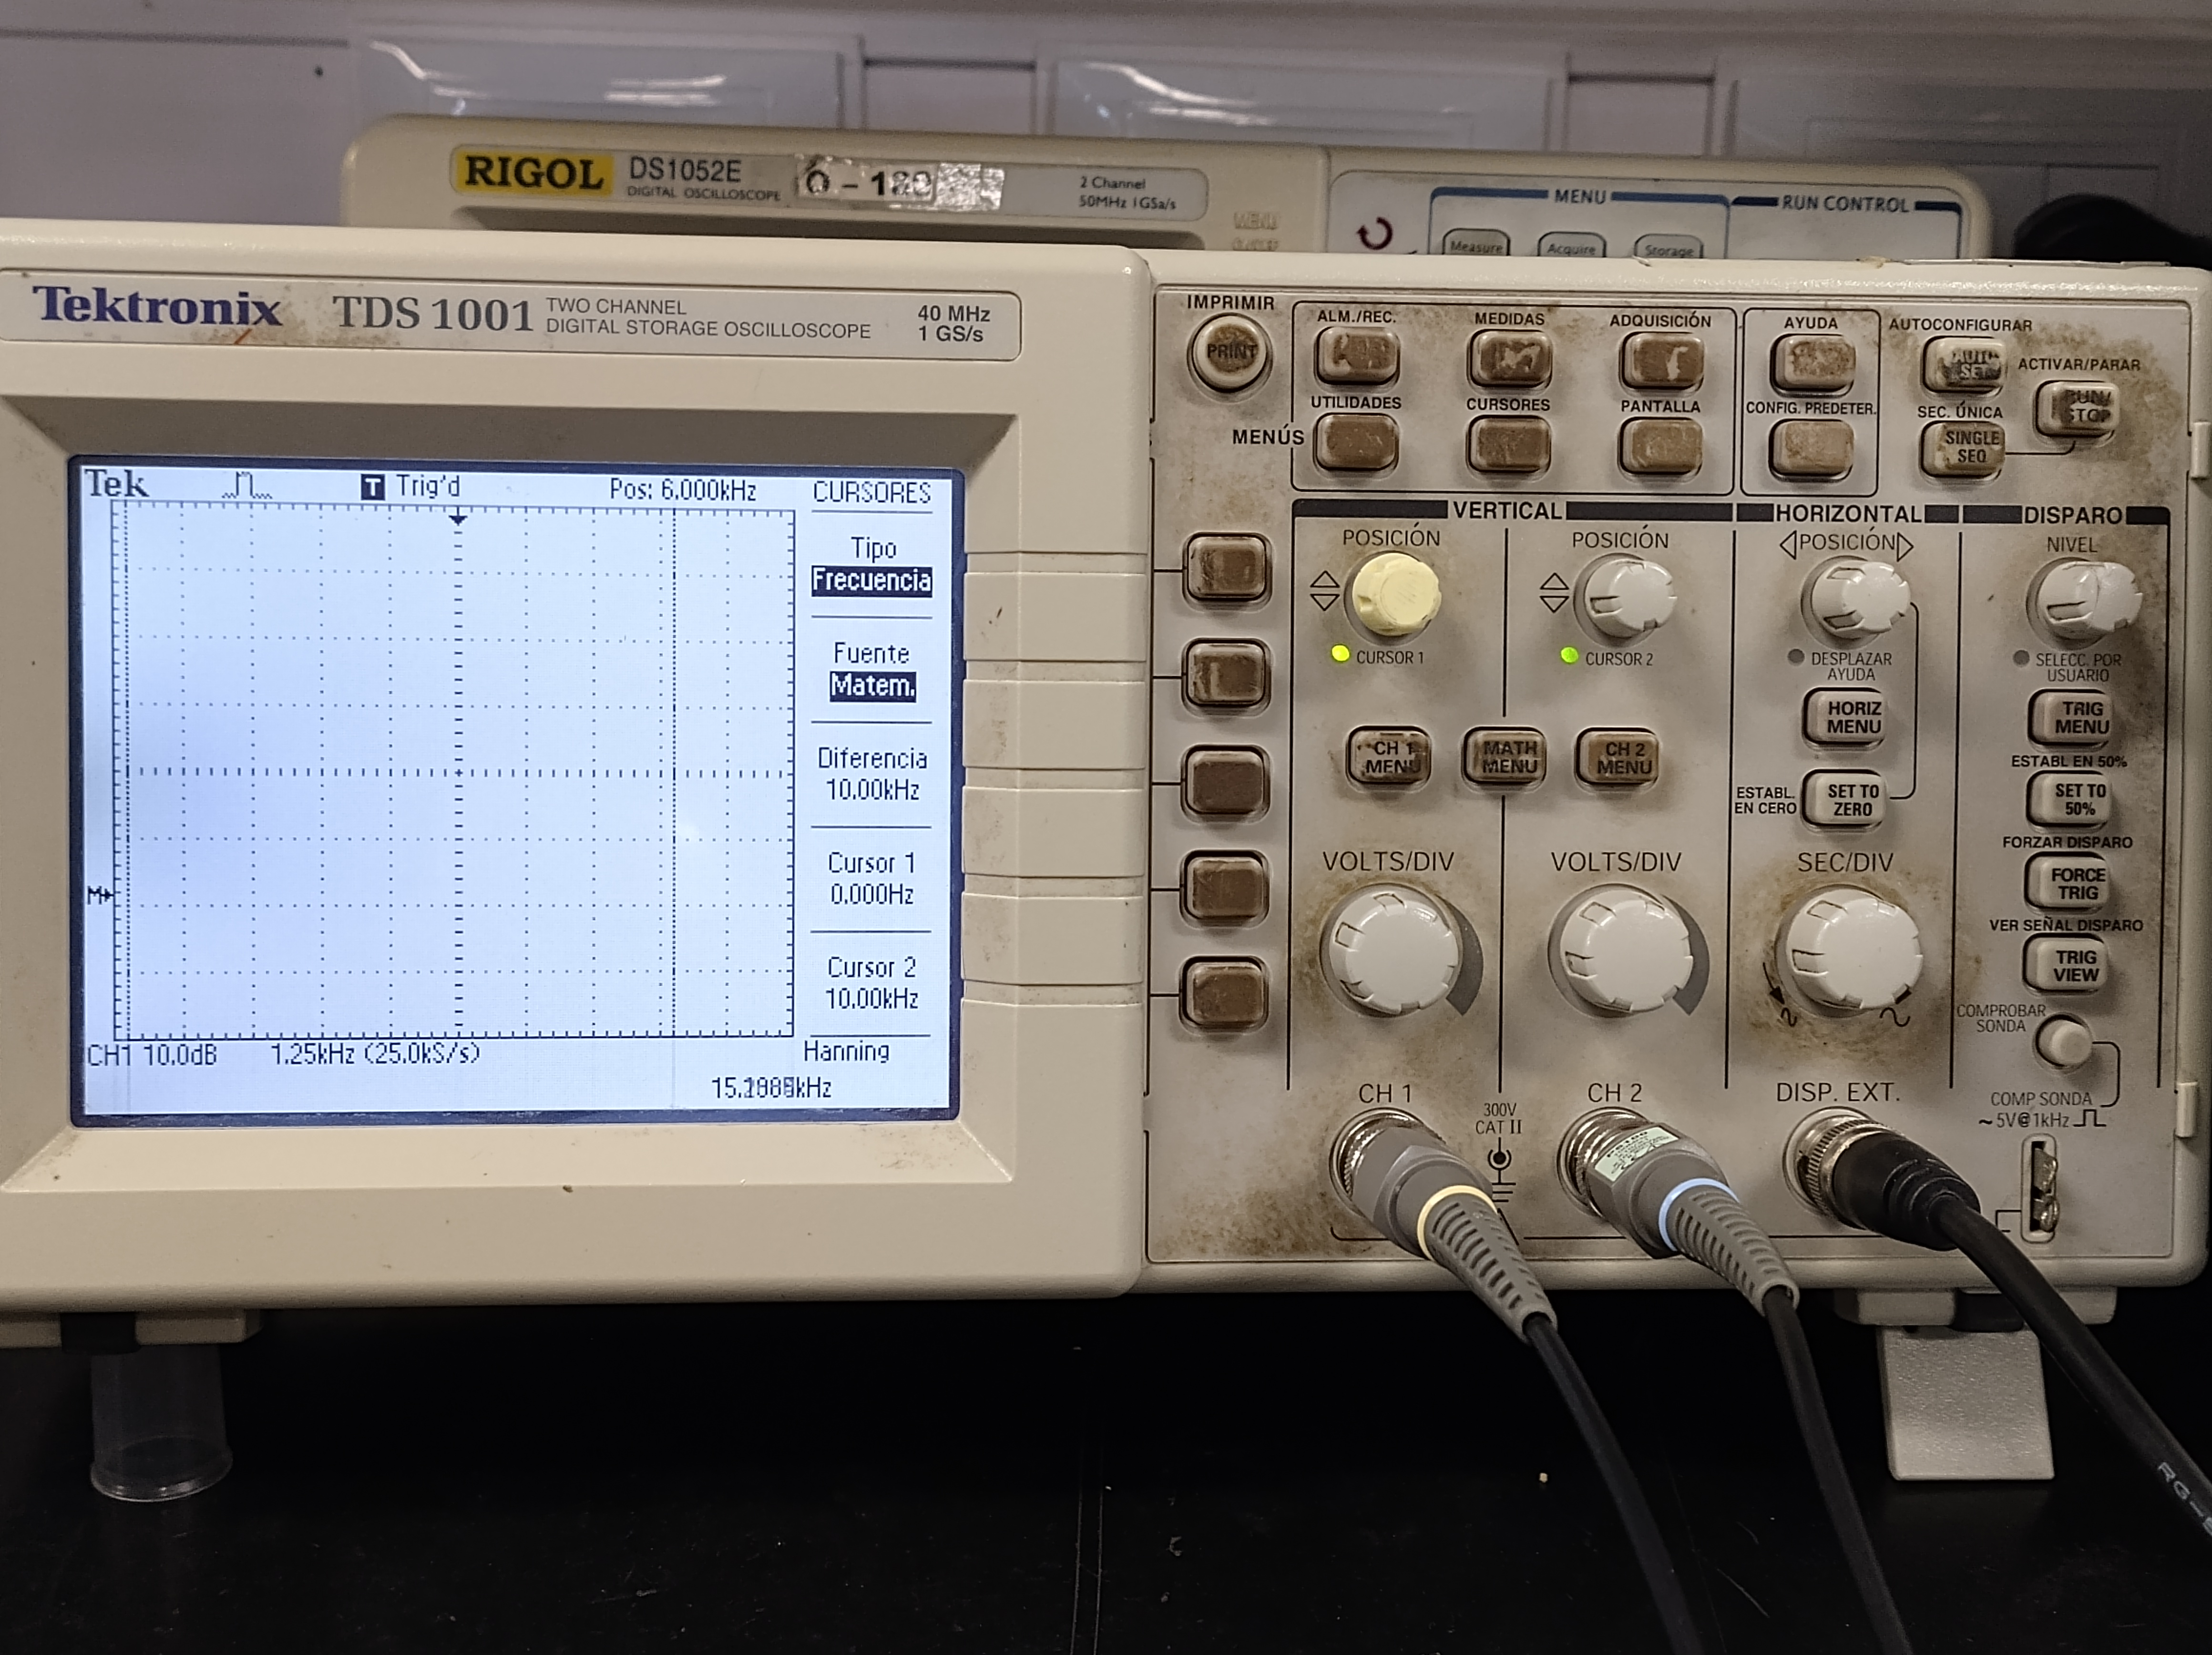
\includegraphics[width=\textwidth]{pictures/osc_tektronix.jpg}
        \caption{Osciloscopio Tektronix TDS 1001.}
        \label{fig.mat:osc_tektronix}
    \end{subfigure}
    \hfill
    \begin{subfigure}[t]{0.48\textwidth}
        \centering
        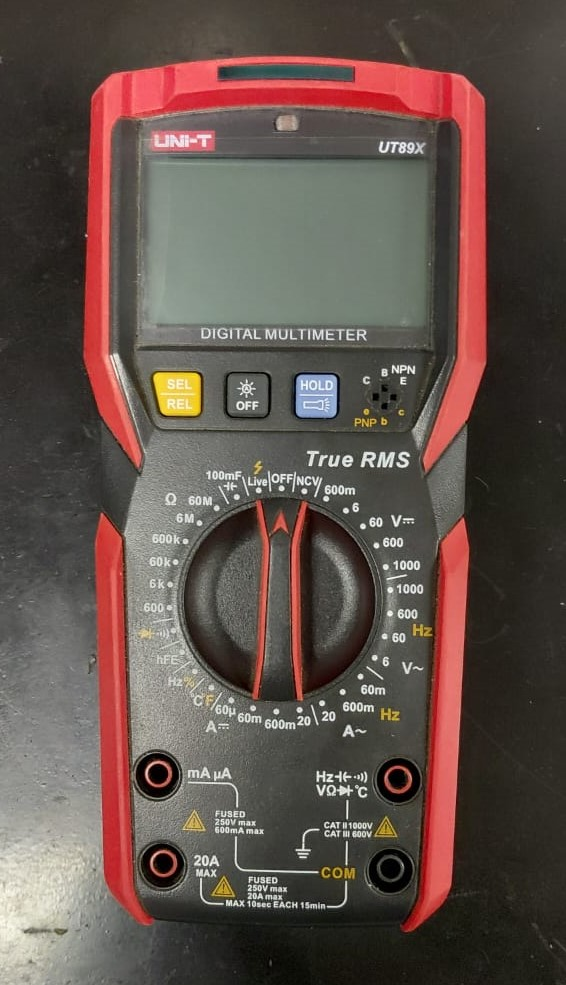
\includegraphics[width=\textwidth]{pictures/multimetro_digital.jpeg}
        \caption{Multímetro digital UT89X.}
        \label{fig.mat:multimetro}
    \end{subfigure}
    \vspace{0.3cm}
    \begin{subfigure}[t]{0.48\textwidth}
        \centering
        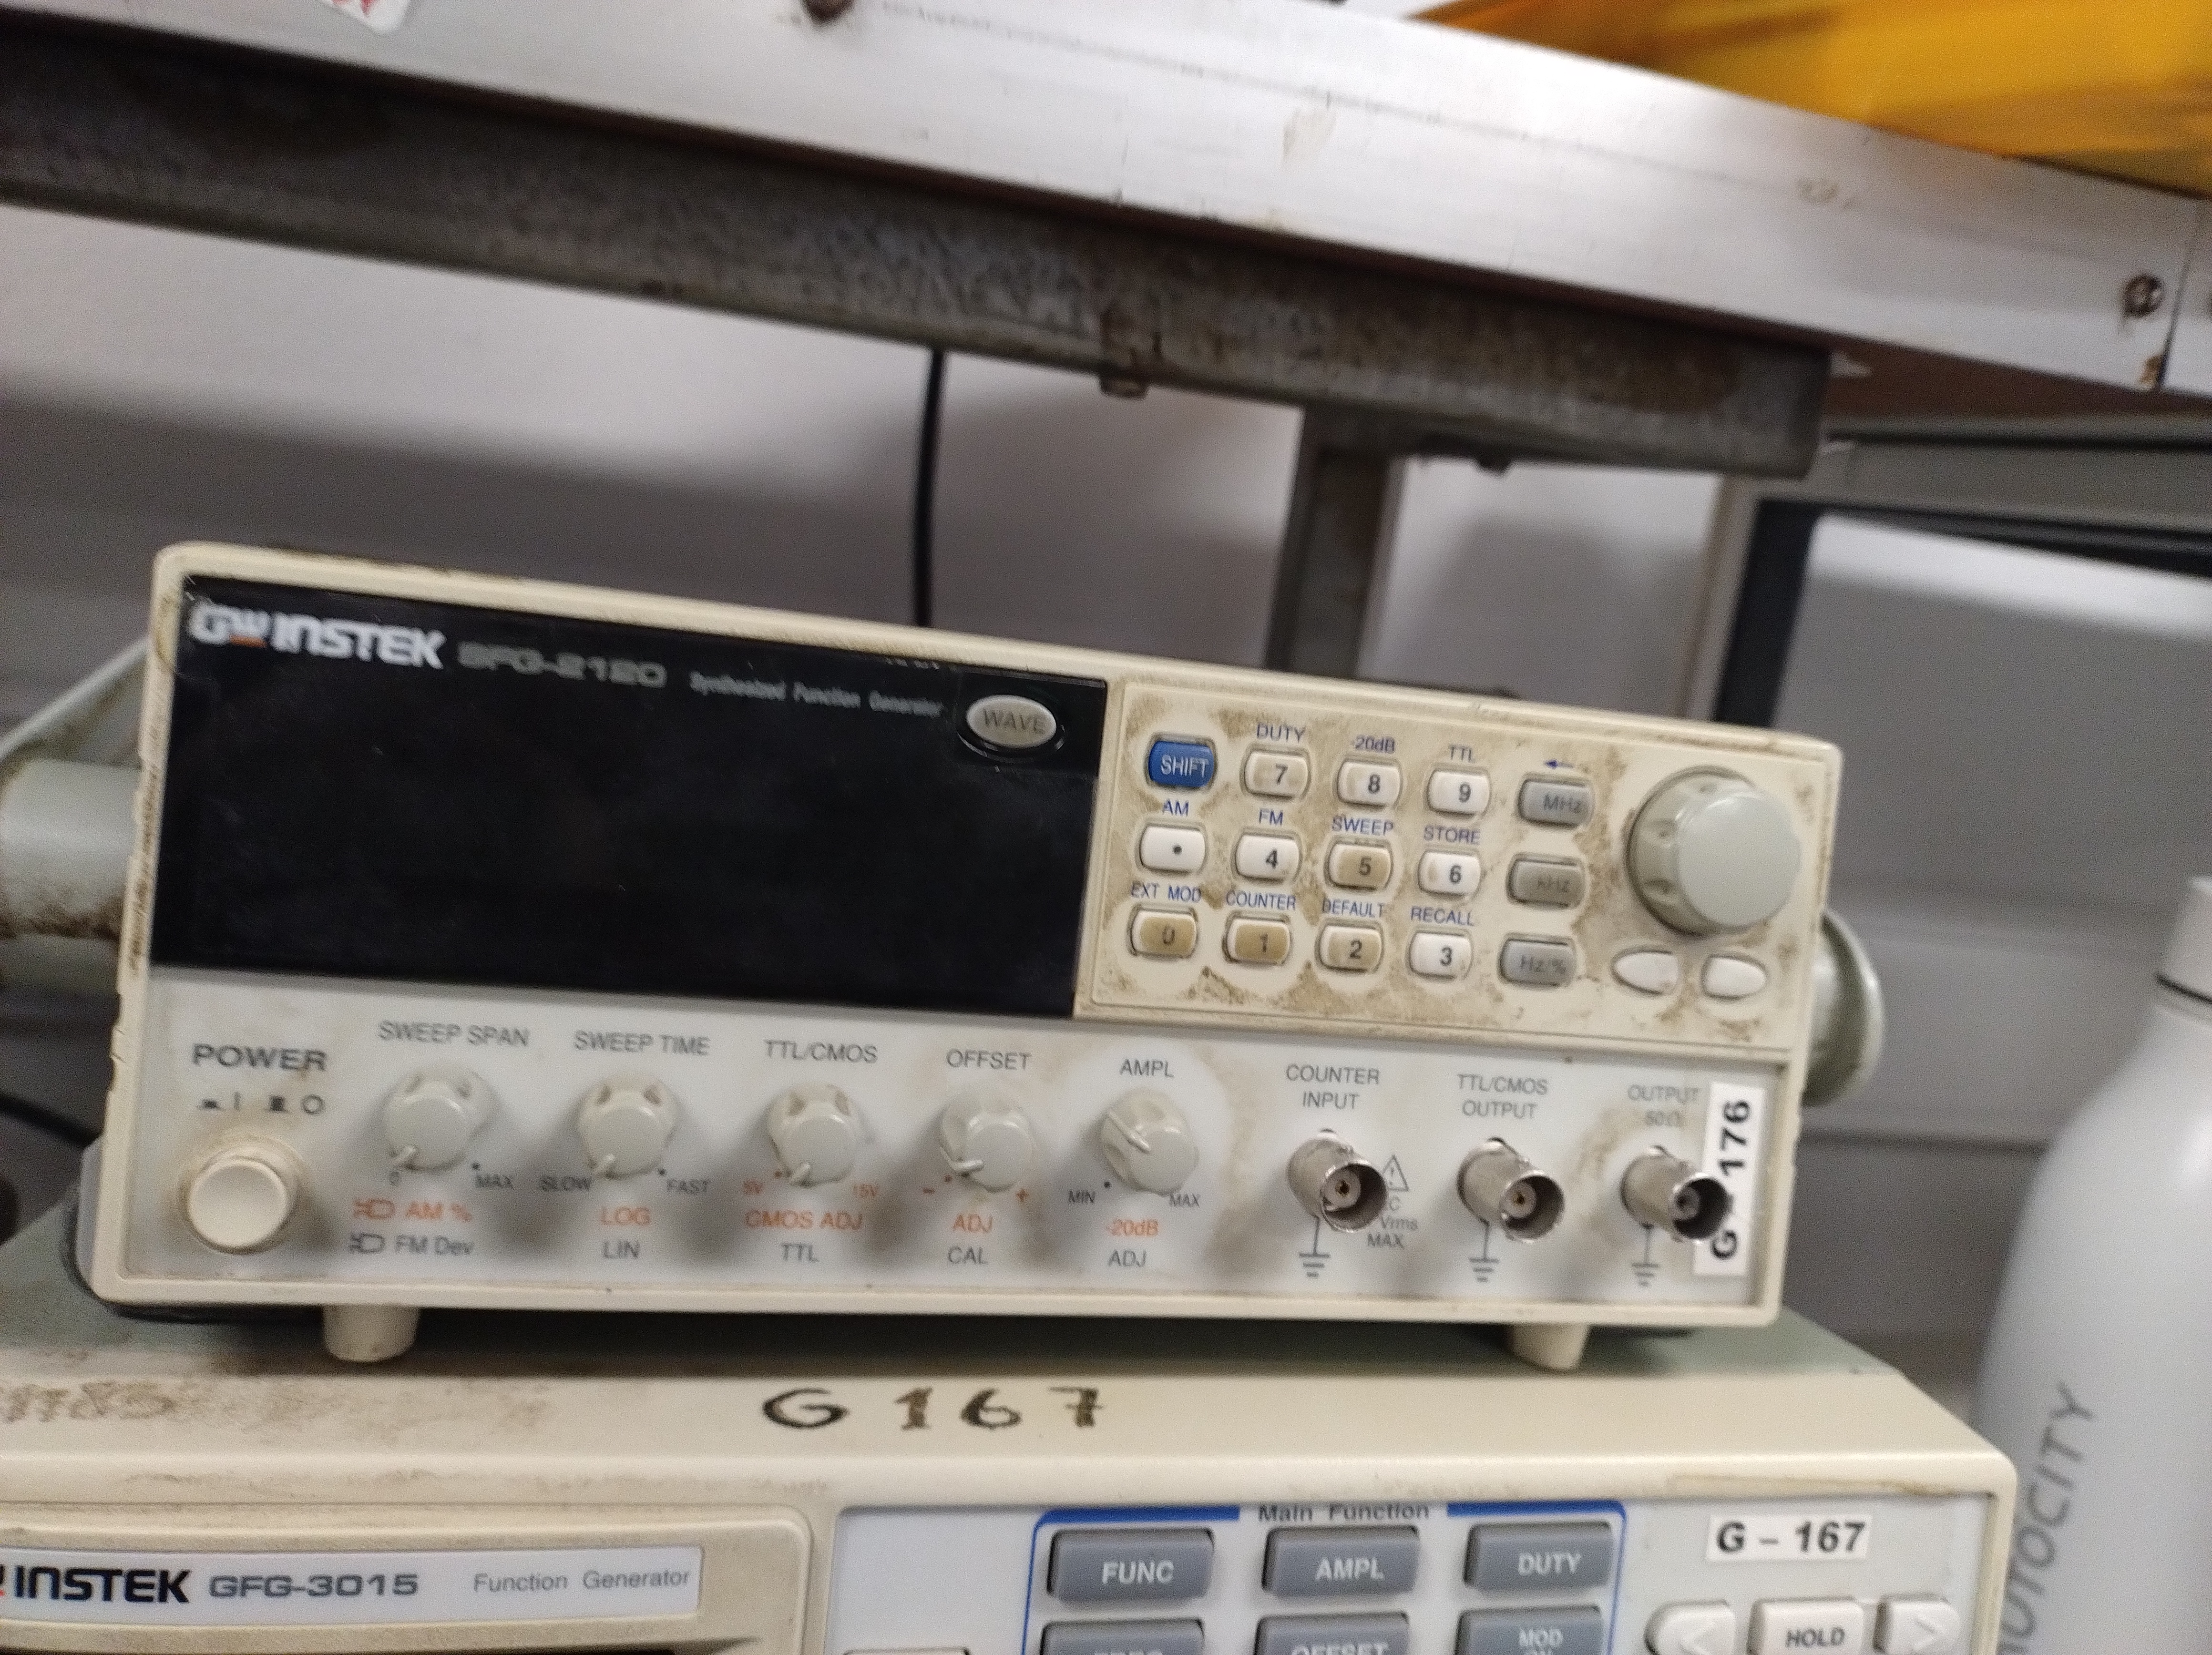
\includegraphics[width=\textwidth]{pictures/gen1.jpg}
        \caption{Generador SFG-2120.}
        \label{fig.mat:gen1}
    \end{subfigure}
    \hfill
    \begin{subfigure}[t]{0.48\textwidth}
        \centering
        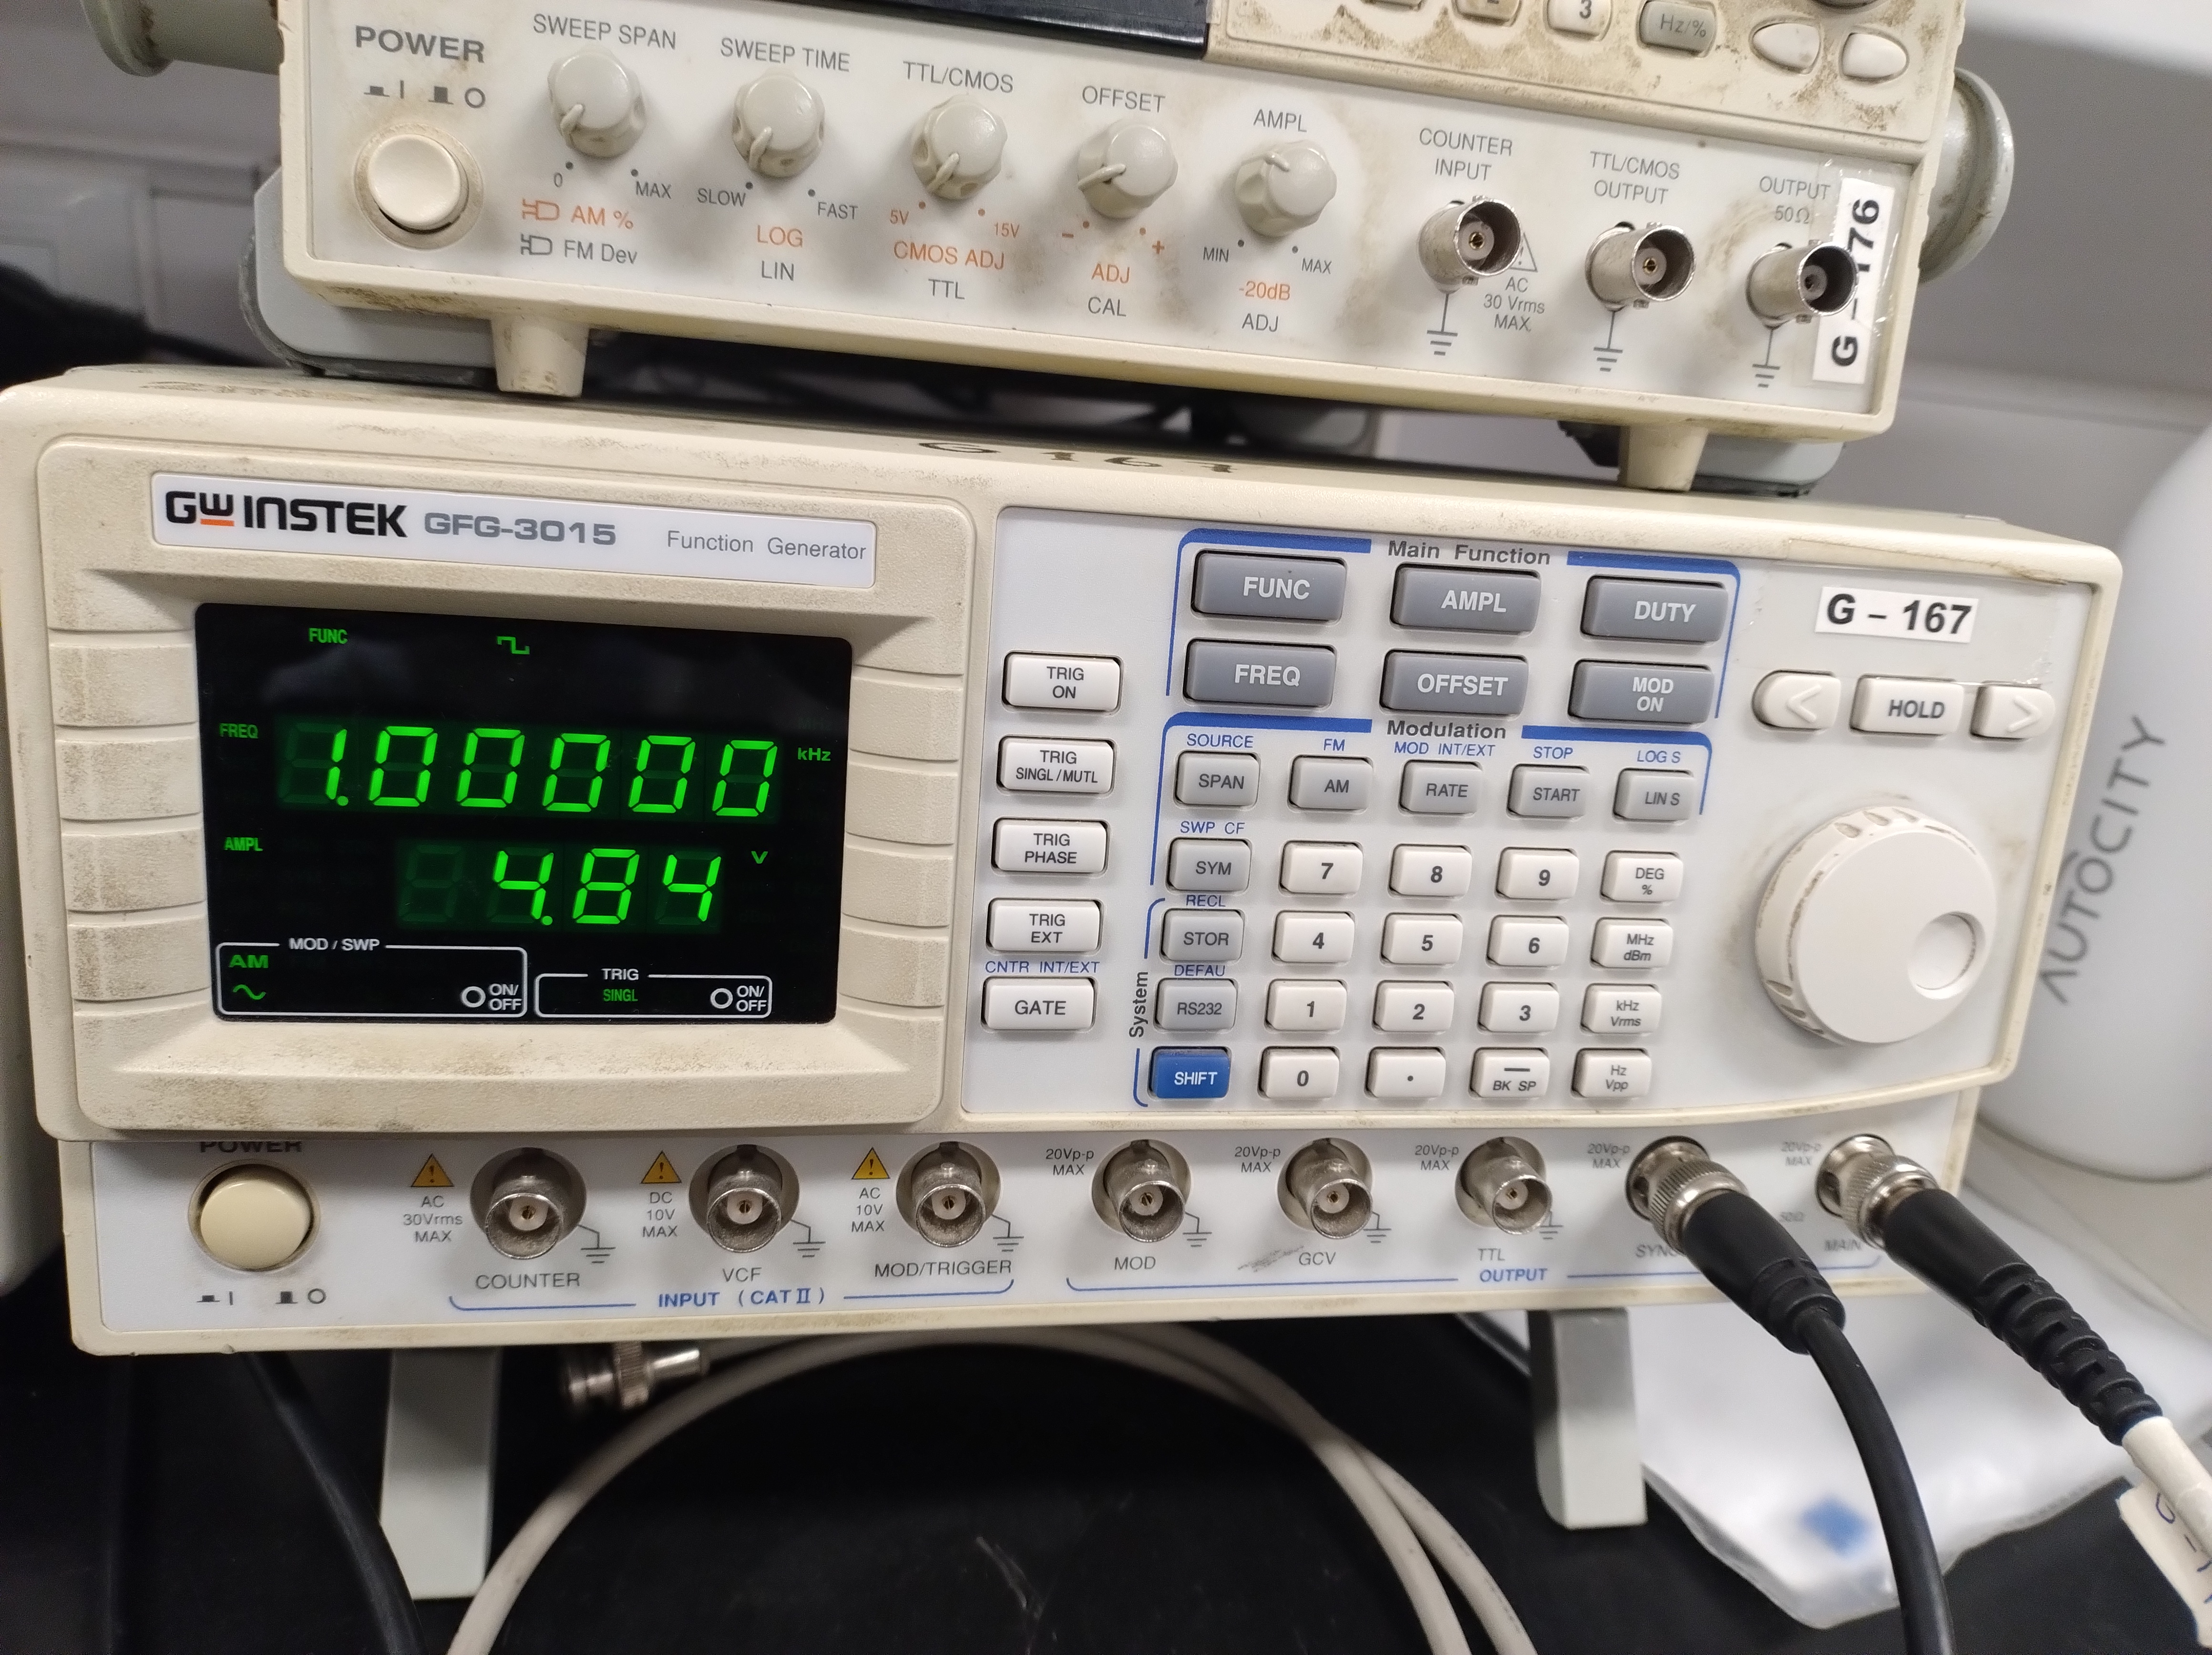
\includegraphics[width=\textwidth]{pictures/gen2.jpg}
        \caption{Generador GFG-3015.}
        \label{fig.mat:gen2}
    \end{subfigure}
    \caption{Instrumental de laboratorio empleado en las actividades experimentales.}
    \label{fig.mat:instrumental_completo}
\end{figure}

\section{Circuitos y Módulos Bajo Prueba}
\begin{itemize}
    \item \textbf{Circuito Modulador de Amplitud (Figura~1 de la consigna):} Módulo pasivo compuesto por dos resistores
    de aislamiento de $R_1 = R_2 = \qty{4.7}{\kilo\ohm}$, un diodo de conmutación rápida para RF ($D_1$) y un circuito
    tanque sintonizado en paralelo ($C = \qty{10}{\nano\farad}$, $L = \qty{1}{\milli\henry}$) sintonizado para resonar en
    torno a $\qty{50}{\kilo\hertz}$.
    \item \textbf{Amplificador Transistorizado de Dos Etapas (Figura~2 de la consigna):} Placa amplificadora clase A con
    jumpers para operar en condición de lazo abierto o a lazo cerrado con realimentación negativa.
    \item \textbf{Potenciómetro de Ajuste ($\qty{1}{\kilo\ohm}$):} Utilizado como atenuador variable en la entrada VCF
    del generador para el control del índice de modulación en frecuencia.
\end{itemize}

\section{Especificaciones de Exactitud del Instrumental}
En el Cuadro~\ref{tab.mat:tolerancias} se resumen las especificaciones de exactitud provistas por los manuales de los
fabricantes para el cálculo de incertidumbres expandidas ($k=2$):

\begin{table}[!ht]
    \centering
    \begin{tabular}{lll}
        \toprule
        \textbf{Instrumento} & \textbf{Magnitud / Función} & \textbf{Tolerancia de Fabricante} \\
        \midrule
        \multirow{3}{*}{Tektronix TDS 1001} 
        & Tensión en el tiempo ($V_{\text{pp}}$, $V_{\text{rms}}$) & $\pm(3\% \cdot \text{lectura} + 0{,}05\,\text{div})$ \\
        & Frecuencia FFT (cursores) & $\Delta f_{\text{bin}} = f_s / 2048 \approx \pm \qty{0.05}{\kilo\hertz}$ \\
        & Nivel FFT (Flattop) & $\pm \qty{0.8}{\dBV}$ \\
        \midrule
        \multirow{2}{*}{UNI-T UT89X}
        & Tensión continua ($V_{\text{DC}}$) & $\pm(0{,}5\% \cdot \text{lectura} + 2\,\text{dígitos})$ \\
        & Tensión alterna ($V_{\text{AC}}$ True RMS) & $\pm(1{,}0\% \cdot \text{lectura} + 3\,\text{dígitos})$ \\
        \bottomrule
    \end{tabular}
    \caption{Tolerancias de catálogo y especificaciones de exactitud del instrumental ($k=2$).}
    \label{tab.mat:tolerancias}
\end{table}
